\section{Persistent Homology by probability}

(preliminary)

While persistence by height allows us to do some basic accounting and comparisons, it is not capturing the graph connectivity questions we are after.  
All transactions at a given time occupy the same set, they are not distinguishable one from the other.
We introduce another construction that lets us try to connect with graph approaches to the analysis.

We will need a notion for distance, and we refer to the cdfs and fits computed in the fit section to do so.

\subsection{Taint Trees}

Persistence works a little bit differently than your intuition might have for probabilities.  
For example a path two-hops deep with .9 connecting the first and .9 connecting the second has probability of .81 of occurring, yet the two txs will already be connected when the filtration parameter reaches .9.  

\subsection{Sampling Paths}

To sample paths each ring has a pymc categorical distribution over the RingCT that we can draw from.  This distribution is also called in calls to the value of a ring or tx.

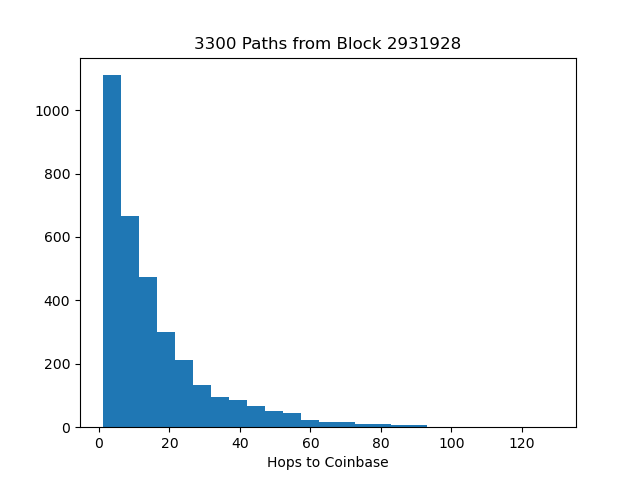
\includegraphics[scale=0.5]{pathstocoinbase} 

\begin{center}
\begin{table}
\begin{tabular}{|c|c|}

\hline
 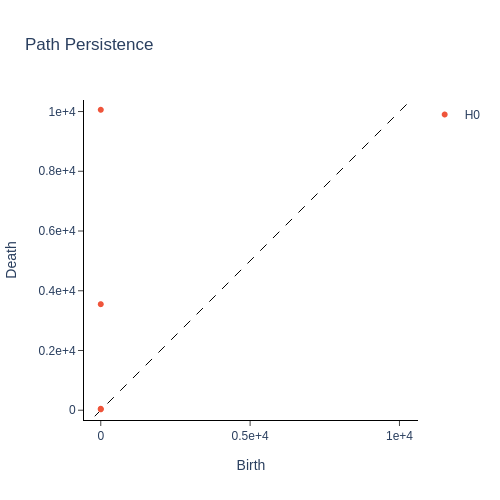
\includegraphics[scale=0.3]{pds_0} & 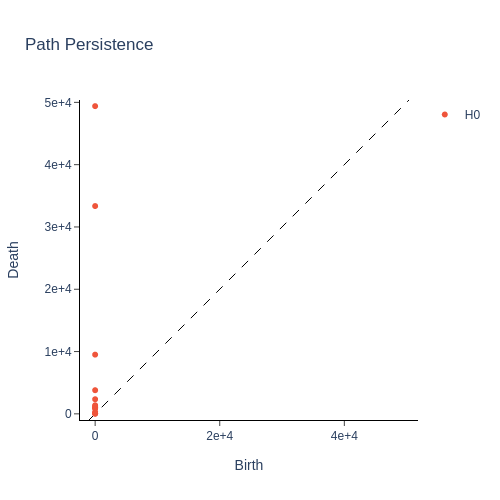
\includegraphics[scale=0.3]{pds_1}  \\ \hline
  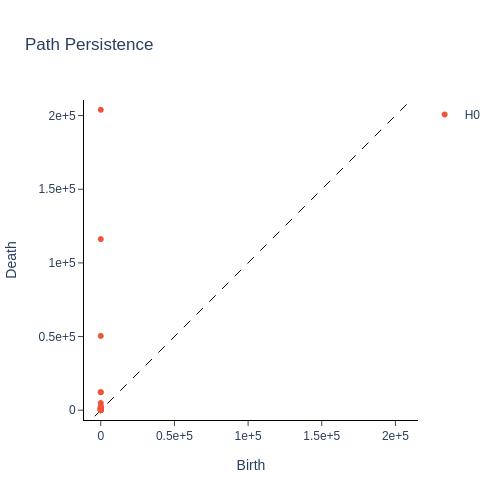
\includegraphics[scale=0.3]{pds_2} & 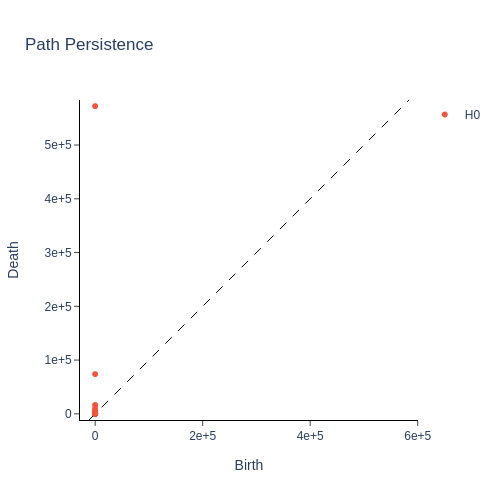
\includegraphics[scale=0.3]{pds_3}  \\ \hline
\end{tabular}
\caption{As the filtration progresses, holes are filled, j}
\end{table}
\end{center}

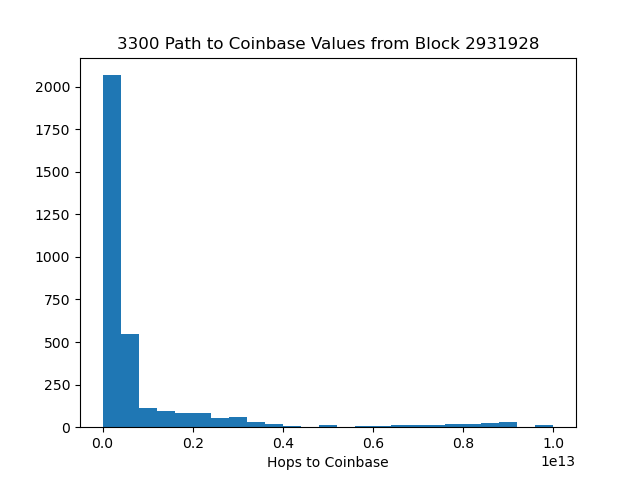
\includegraphics[scale=0.5]{valscoinbase} 